\documentclass{./packages/rs/rsproca}
\graphicspath{{./images/}}
% *** Do not adjust lengths that control margins, column widths, etc. ***

%%%%%%%%%%% Defining Enunciations  %%%%%%%%%%%
\newtheorem{theorem}{\bf Theorem}[section]
\newtheorem{condition}{\bf Condition}[section]
\newtheorem{corollary}{\bf Corollary}[section]
%%%%%%%%%%%%%%%%%%%%%%%%%%%%%%%%%%%%%%%%%%%%%%%


\begin{document}

%%%% Article title to be placed here
\title{Shock Heating in Numerical Simulations of Kink-unstable Coronal Loops}

\author{%%%% Author details
M. R. Bareford and A. W. Hood}

%%%%%%%%% Insert author address here
\address{School of Mathematics and Statistics,\\University of St Andrews, North Haugh, St Andrews, Fife KY16 9SS, UK}

%%%% Subject entries to be placed here %%%%
\subject{Solar system (169), Computer modelling and simulations, Plasma physics}

%%%% Keyword entries to be placed here %%%%
\keywords{Coronal heating, Magnetic kink instability, Slow mode shocks}

%%%% Insert corresponding author and its email address}
\corres{M. R. Bareford\\
\email{michael.bareford@epcc.ed.ac.uk}}

\begin{abstract}
An analysis of the importance of shock heating within coronal magnetic fields has hitherto been a neglected area of study. We present new results obtained from nonlinear magnetohydrodynamic (MHD) simulations of straight coronal loops. This work shows how the energy released from the magnetic field, following an ideal instability, can be converted into thermal energy, thereby heating the solar corona. Fast dissipation of magnetic energy is necessary for coronal heating and this requirement is compatible with the time scales associated with ideal instabilities. Therefore, we choose an initial loop configuration that is susceptible to the fast-growing kink, an instability that is likely to be created by convectively-driven vortices, occurring where the loop field intersects the photosphere (i.e., the loop footpoints). The large-scale deformation of the field caused by the kinking creates the conditions for the formation of strong current sheets and magnetic reconnection, which have previously been considered as sites of heating, under the assumption of an enhanced resistivity. However, our simulations indicate that slow mode shocks are the primary heating mechanism, since, as well as creating current sheets, magnetic reconnection also generates plasma flows that are faster than the slow magnetoacoustic wave speed.
\end{abstract}

\begin{fmtext}
\end{fmtext}

\maketitle

\section{Introduction}
\label{sec_Introduction}

The energy that heats the solar corona is thought to be released from magnetic fields that cover thousands of kilometres rising from and closing back down in the photosphere. As a consequence of these megametre scales, and as a result of the near-perfect conductivity within the solar atmosphere, coronal magnetic fields diffuse slowly ($t_{\mathrm{d}}\,{\approx}\,10^3\,\mathrm{yr}$). This leads to the important property that the magnetic field is \textit{frozen} into the plasma, thereby allowing convective motions at the photospheric boundaries to continually reconfigure coronal magnetic fields. Hence, the work done by convective flows is stored within the corona as free magnetic energy. Since the time scale associated with photospheric convection is long compared to the Alfv\'en time, the coronal magnetic field can regain equilibrium each time more energy is stored. This means that when an instability does eventually occur, the amount of energy accumulated is sufficient to heat the surrounding plasma to million degree temperatures. The radiation associated with this heating reveals the general topology of coronal magnetic fields, which, are commonly observed as bundles of discrete coronal loops above solar active regions.

This paper is concerned with how an ideal kink instability [1-4] --- that we assume is the eventual consequence of continual photospheric driving --- can lead to the heating of a coronal loop. Many ideal instabilities generate current sheets, which when accompanied by resistive effects, allow a change in magnetic topology, increasing the amount of energy that can be released. We investigate the ideal kink [5] since its growth rate is fast enough to match flare-like time scales. In addition, there is a substantial body of work [6-11], based on numerical simulations, that demonstrates how the kink instability creates sheets of high current density, facilitating magnetic reconnection. 

The mechanism whereby magnetic energy is converted into heat has often been attributed to Ohmic dissipation [10-16]; usually, this is implemented by \textit{switching on} an increased resistivity whenever the current exceeds some critical value. However, recent work involving coronal loop simulations [17], has revealed a strong connection between plasma heating and the shocks resulting from a kink instability. This is perhaps not surprising, since for several decades now, slow mode shocks [18] have been known to be an important feature of Petschek (or fast) reconnection [19], where the shortening of the current sheet allows shocks to form in the outflow region, enhancing the diffusion of magnetic energy. Much research has been done to investigate the critical parameters responsible for fast reconnection [20-22]. In addition, other workers have observed slow mode shocks within large-scale numerical simulations of the solar environment [23-25], and even observational data has provided strong evidence for shocks located at flare sites [26]. A common feature of numerical reconnection experiments is the use of a driven (or perturbed) current sheet, and, for models of the solar atmosphere, reconnection results from allowing magnetic flux to rise into the corona. In this work, we show that the conditions for reconnection and slow mode shocks can also occur when a coronal loop undergoes a kink instability. Since coronal fields are line-tied at the photospheric boundary, vortical motions associated with convection will repeatedly twist the loop until it becomes kink unstable [27,28].

The paper is structured as follows. Section \ref{sec_LoopModel} describes the loop model in terms of its initial magnetic field. Next, we present the numerical code and focus on how well it performs with regard to shock capturing. We also discuss an improved implementation of anomalous resistivity, where, instead of an arbitrary constant, we use a variable critical current based on local plasma conditions. Our aim here is to rule out the possibility of Ohmic heating being underestimated in numerical experiments. \mbox{Section \ref{sec_NumericalResults}} discusses the simulation results: specifically, when and where energy is released from the magnetic field, and how this energy is thermalised. Lastly, the results are summarised and our conclusions are given. The instructions, scripts and source code required to reproduce the results presented in this paper are held in an online GitHub repository [29].

\section{Loop model}
\label{sec_LoopModel}

A coronal loop is modelled as a straight cylinder with a loop axis that is initially coincident with the $z$-axis. Assuming the magnitude of the magnetic field on the axis, $B_0$, as a typical field strength and the radius of the cylinder, $R_0$, as a typical length, we use the magnetic field equations given by Hood et al. [13] to define a dimensionless initial loop equilibrium that has \textit{zero} net current:
\begin{align}\begin{split}
\label{eqn_btheta}
B_{\theta} &= \lambda r \Big(1 - r^2\Big)^{3}\,,\\
\end{split}\end{align}
\begin{align}\begin{split}
\label{eqn_bz}
B_{z} &= \Bigg[\frac{\lambda^2}{7}\Bigg(\Big(1-r^2\Big)^{7} - 1\Bigg) - \lambda^2 r^2 \Big(1-r^2\Big)^{6} + 1\Bigg]^{\frac{1}{2}}\,,
\end{split}\end{align}
where $r$ is in the range $0\,{\leq}\,r\,{\leq}\,1$, and $\lambda$ is a constant. The somewhat complicated expression for $B_z$ is actually derived from $\vec{B}\,{=}\,B_{\theta}(r)\hat{\theta} + B_z(r)\hat{z}$ and $(\nabla\times\vec{B})\,{\times}\,\vec{B}\,{=}\,0$ (i.e., a force-free equilibrium is assumed). Thus, an expression for the ratio of current density to magnetic field, $\alpha\,=\,(\vec{j}\cdot\vec{B})$/$(|\vec{B}|^{2})$, which is continuous throughout the loop volume, can be determined,
\begin{align}\begin{split}
\label{eqn_alpha}
\alpha &= \frac{1}{B_z} 2 \lambda \Big(1 - r^2\Big)^{2}\Big(1 - 4r^2\Big)\,.
\end{split}\end{align}
    
\begin{figure}[!h]
  \centering
  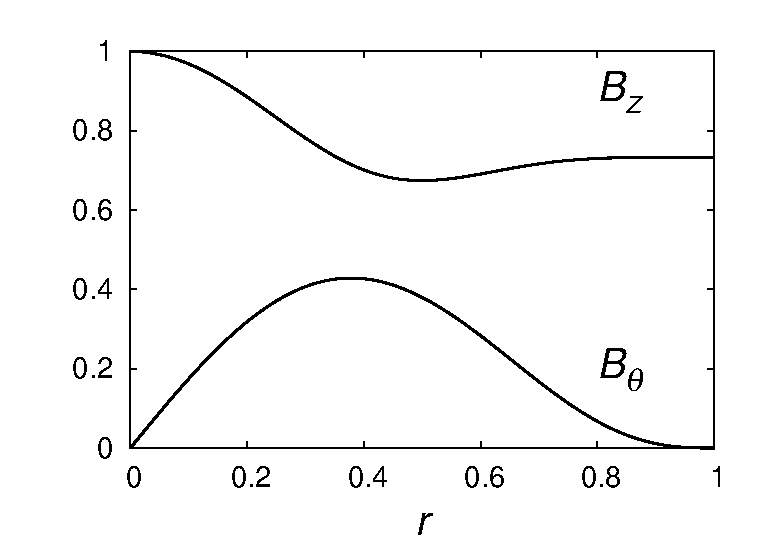
\includegraphics[scale=0.47]{./gnuplot/b}
  \hspace{10pt}
  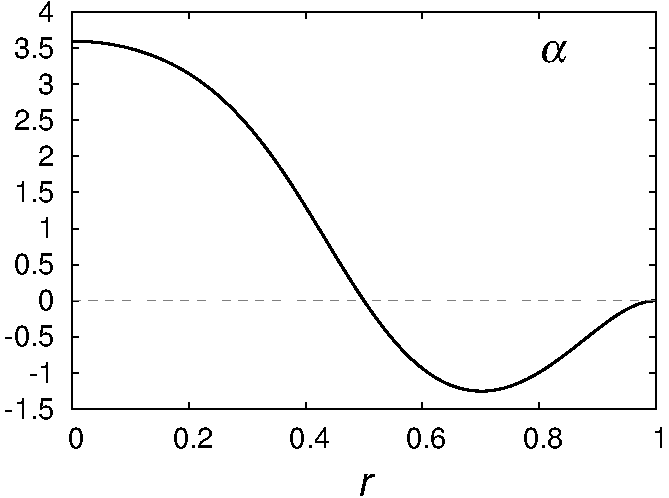
\includegraphics[scale=0.47]{./gnuplot/alpha}
  \caption{\small{The initial loop field produced by $\lambda\,{=}\,1.8$ (left) and the derived continuous $\alpha$-profile (right).}}
  \label{fig_field_alpha}
\end{figure}

These expressions, valid for $0\,{\le}\,r\,{\le}\,1$, are illustrated by Figure \ref{fig_field_alpha}. Outside the loop, $B_z\,{=}\,\sqrt{1 - \lambda^2/7}$ and $B_{\theta}\,{=}\,\alpha\,{=}\,0$. The footpoints of the loop are located at the $z$-limits ($|z|\,{=}\,10$) and so the loop apex is at $z\,{=}\,0$ (the azimuthal plane is synonymous with the $x$-$y$ plane). The radial boundary is defined by the extent of the azimuthal field; this extent is itself an outcome of the spatial scale of the convective motions that generate the currents (and thereby azimuthal field). Essentially, localised footpoint motions will always define a loop that has zero net current. This loop configuration is linearly kink unstable when $\lambda\,{\ge}\,1.62$. We use $\lambda\,{=}\,1.8$, since it is fully unstable, and allows us to compare our results with previous work [13,30].

At the start of the simulation a weak perturbation is applied to the loop,
\begin{align}\begin{split}
\label{eqn_perturbed_radial_velocity}
v_r &= \frac{1}{10^{4}}\,e^{-r^2\big(1+64r^6\big)}\,\Bigg[\cos{\Bigg(\frac{\pi}{L} z\Bigg)}\cos\big(kz-\theta\big)\Bigg]\,,
\end{split}\end{align}
where $v_r$ is the radial component of the perturbed velocity, $L\,{=}\,20$ is the loop length, $k\,{=}\,0.3\pi$ is the wave number, and $\theta\,{=}\,\arctan(y/x)$. This disturbance initiates the kink instability and its form is constructed such that the amplitude of the perturbation falls off quickly with radius.

\section{Numerical code}
\label{sec_NumericalCode}
The numerical simulations are performed using a 3D MHD code called LARE3D [31]. This code follows a \textbf{La}grangian \textbf{re}map scheme, hence its name. Essentially, the Lagrangian part, which is done using a second-order accurate predictor-corrector method, deforms the grid such that it moves with the plasma. The advantage of this technique is that additional physics (e.g., shock capturing) can easily be incorporated into the code. The remap stage involves the mapping of the plasma propertie back to the original Cartesian grid; monotonicity is preserved through the use of Van Leer [32] gradient limiters.

LARE3D solves the following resistive MHD equations,
\begin{align}\begin{split}
\label{eqn_lare_mhd_mass}
\frac{\partial\rho}{\partial t} &= -\nabla\cdot(\,\rho\vec{v}\,)\,,\\
\end{split}\end{align}
\begin{align}\begin{split}
\label{eqn_lare_mhd_force}
\frac{\partial}{\partial t}\big(\,\rho\vec{v}\,\big) &= -\nabla\cdot(\,\rho\vec{v}\vec{v}\,)\,\,+\,\,\frac{1}{\mu_0}\Big(\,\nabla\times\vec{B}\,\Big)\times\vec{B}\,\,-\,\,\nabla{P}\,\,+\,\,\nabla\cdot{\vec{\sigma}}\,,\\
\end{split}\end{align}
\begin{align}\begin{split}
\label{eqn_lare_mhd_induction}
\frac{\partial\vec{B}}{\partial t} &= \nabla\times\Big(\,\vec{v}\times\vec{B}\,\Big)\,\,-\,\,\nabla\times\Bigg(\eta\frac{\nabla\times\vec{B}}{\mu_0}\Bigg)\,,\\
\end{split}\end{align}
\begin{align}\begin{split}
\label{eqn_lare_mhd_energy}
\frac{\partial}{\partial t}\big(\,\rho\epsilon\big) &= -\nabla\cdot(\,\rho\epsilon\vec{v}\,)\,\,\,-\,\,P\,\nabla\cdot\vec{v}\,\,+\,\,\eta J^{\,2}\,\,+\,\,\vec{\varepsilon}\,\vec{\sigma}\,,
\end{split}\end{align}
with specific energy density,
\begin{align}\begin{split}
\label{eqn_lare_mhd_epsilon}
\epsilon &= \frac{P}{(\gamma-1)\,\rho}\,,
\end{split}\end{align}
where $\rho$ is the mass density, $\vec{v}$ is the plasma velocity, $\vec{B}$ the magnetic field, $P$ the thermal pressure, $\eta$ is the resistivity, $J$ is the current density, $\gamma\,{=}\,5/3$ is the ratio of specific heats, and $\mu_0$ is the magnetic permeability. The last terms of equations \ref{eqn_lare_mhd_force} and \ref{eqn_lare_mhd_energy} feature tensors, and are required to simulate the effect of hydrodynamic shocks; these are defined in \mbox{Section 3 \ref{sec_NumericalCode_ShockResolution}}.

We normalise the variables in the MHD equations using dimensional values suitable for a coronal active region:
\begin{align}\begin{split}
r_{\ast} &= \frac{r}{R_0}\,,\,\,\,\,\,\,\rho_{\ast}\,\,=\,\,\frac{\rho}{\rho_0}\,,\,\,\,\,\,\,T_{\ast}\,\,=\,\,\frac{T}{T_0}\,,\,\,\,\,\,\,B_{\ast}\,\,=\,\,\frac{B}{B_0}\,,
\end{split}\end{align}
where asterisk subscripts denote the normalised MHD variables. For example $R_0\,{=}\,1\,\mathrm{Mm}$ is the loop radius. The density and temperature are initially uniform ($\,\rho_0\,{=}\,1.67\,{\times}\,10^{-12}\,\mathrm{kg}\,\mathrm{m}^{-3}$ and $T_0\,{=}\,20\,000\,\mathrm{K}$), and $B_0\,{=}\,0.005\,\mathrm{T}$ is the initial axial field strength. Thus, at $t\,{=}\,0$, the plasma is dominated by the magnetic field: plasma-$\beta$ is of order $10^{-5}$. Other variables are expressed in a similar manner;
\begin{align}\begin{split}
L_{\ast} &= \frac{L}{R_0}\,,\,\,\,\,\,\,t_{\ast}\,\,=\,\,\frac{t}{t_{\mathrm{A}}}\,,\,\,\,\,\,\,v_{\ast}\,\,=\,\,\frac{v}{v_{\mathrm{A}}}\,,\,\,\,\,\,\,P_{\ast}\,\,=\,\,\frac{P}{P_0}\,,
\end{split}\end{align}
where ${L}\,{=}\,20\,R_0$ is the loop length, $t_{\mathrm{A}}\,{=}\,R_0/v_{\mathrm{A}}$ is the radial Alfv{\'e}n transit time, $v_{A}\,{=}\,B_0/\sqrt{\mu_0\rho_0}$ the Alfv{\'e}n speed, and $P_0\,{=}\,B_0^{\,2}/\mu_0$ the magnetic pressure. Hence, the length becomes $20\,\,\mathrm{Mm}$, $t_{\mathrm{A}}\,{\approx}\,0.3\,\mathrm{s}$ and $v_{\mathrm{A}}\,{\approx}\,3.4\,\,\mathrm{Mm}\,\mathrm{s}^{-1}$. 

The computational domain is a 3D staggered grid: physical variables are not calculated at the same place for each cell in the domain, which improves numerical stability and allows conservation laws to be included in the computation. The domain size is \mbox{$L_x\,{=}\,L_y\,{=}\,4$ (-2:+2)} and $L_z\,{=}\,20$ (-10:+10). The loop is line-tied at $z\,{=}\,{-}\,10,\,+10$, which means, at those $z$-coordinates, the velocity components are set to zero. The velocity components are also zero at the boundaries for the other two directions. In addition, the normal derivatives of magnetic field, energy and density are zero at all boundaries. The simulations were run at three grid resolutions, \mbox{$128^{\,2}\,{\times}\,256$ (low)}, $256^{\,2}\,{\times}\,512$ (medium) and $512^{\,2}\,{\times}\,1024$ (high). Unless stated otherwise all figures shown in Section \ref{sec_NumericalResults} are taken from the medium resolution run. Using three different resolutions allows us to investigate if the shock heating is real or merely an artefact of inadequate spatial resolution.


\subsection{Shock resolution}
\label{sec_NumericalCode_ShockResolution}
The dominance of shock heating within simulations of kink-unstable loops [12,13,17] requires us to explain how this important mechanism is implemented. LARE3D uses shock viscosity [33] to capture the heating effect of shocks, which is implemented by adding an extra term to the energy equation. This term is expressed as the product of the rate of strain tensor,
\begin{align}\begin{split}
\label{eqn_lare_strain_tensor}
\varepsilon_{ij} &= \frac{1}{2}\Bigg(\frac{\partial\,v_i}{\partial\,x_j}\,\,+\,\,\frac{\partial\,v_j}{\partial\,x_i}\Bigg)\,,
\end{split}\end{align}
and the shock tensor,
\begin{align}\begin{split}
\label{eqn_lare_shock_viscosity_tensor}
\sigma_{ij} &= \rho\,l_{\mathrm{s}}\,\Big(\nu_1\,c_{\mathrm{ms}}\,\,+\,\,\nu_2\,l_{\mathrm{s}}\,|\,s\,|\Big)\,\Bigg(\varepsilon_{ij}\,\,-\,\,\frac{1}{3}\,\delta_{ij}\,\nabla\cdot\vec{v}\Bigg)\,,
\end{split}\end{align}
where $\vec{v}$ is the velocity, $c_{\mathrm{ms}}\,{=}\,\sqrt{c_{\mathrm{s}}^2 + v_{\mathrm{A}}^2}$ is the magnetosonic speed, $l_{\mathrm{s}}$ is the distance across a grid cell in the direction normal to the shock front, $s$ is a similarly localised strain rate (the subscripts $i$ and $j$ denote the different spatial coordinates), and the shock viscosity coefficients $\nu_1\,{=}\,0.1$ and $\nu_2\,{=}\,0.5$ are constants. The terms within the rightmost set of brackets in equation \ref{eqn_lare_shock_viscosity_tensor} evaluate to zero when a cell undergoes uniform compression/expansion or rigid rotation. If we approximate these terms (and $|s|$) by $\nabla \vec{v}/l_{\mathrm{s}}$,
\begin{align}\begin{split}
\label{eqn_lare_shock_viscosity_tensor_simple}
\sigma_{ij} &\approx \nu_1\,c_{\mathrm{ms}}\,\rho\,(\nabla\vec{v})\,\,+\,\,\nu_2\,\rho\,(\nabla\vec{v})^2\,,
\end{split}\end{align}
where the linear term damps out the non-physical oscillations caused by finite differencing in the numerical code and also dissipates kinetic energy. More of the dissipation is handled by the quadratic term as the shock increases in strength. The \textit{form} of equation (\ref{eqn_lare_shock_viscosity_tensor_simple}) can be derived from the Rankine-Hugoniot jump conditions; furthermore if one neglects terms higher than second order it is possible to obtain values of $1$ and $2/3$ for $\nu_1$ and $\nu_2$ respectively. However, equation (\ref{eqn_lare_shock_viscosity_tensor}) is expressed in terms of tensors, which have been included in such a way so as to prevent non-physical results under MHD conditions. The energy dissipation associated with each grid cell depends on the level of non-uniform shearing. Note, there is no \textit{real} viscosity in the simulations presented here. The viscosity part of shock viscosity comes from the mathematical form used to capture shock heating. Shocks create steep velocity gradients and the heating implied by these gradients is captured by the viscous-like terms of Equations \ref{eqn_lare_shock_viscosity_tensor} and \ref{eqn_lare_shock_viscosity_tensor_simple}.

Arber et al. [31] tested the shock-capturing capabilities of the LARE code (with $\nu_1\,{=}\,0.1$ and $\nu_2\,{=}\,1$) by running a series of numerical experiments based on the work of Brio \& Wu [34]. A shock is initialised by having discontinuities in density, pressure and magnetic field along some boundary that divides a 2D plane. We have repeated these tests using the values for the shock viscosity coefficients given here ($\nu_1\,{=}\,0.1$, $\nu_2\,{=}\,0.5$) at a resolution of $256\times256$. As with Arber et al., we obtained results that agreed closely with those of Brio \& Wu. Such comparisons are useful because Brio \& Wu used a second-order upwind scheme, which avoids the problem of false oscillations behind the shock front.

\subsection{Critical current density}
\label{sec_NumericalCode_CriticalCurrentDensity}

In numerical simulations of coronal loops, the background resistivity is usually set to zero in order to represent the near perfect conductivity of the coronal environment. Ohmic heating only occurs when an anomalous (non-zero) resistivity is applied in response to the current density reaching a threshold value. Using an arbitrary value for the threshold is problematic when trying to determine the significance of Ohmic heating compared to other forms of heating. A high current density (at least double that of the maximum initial value) is assumed to be caused by a reduction in the local conductivity, which either arises from a small-scale turbulent process or is a consequence of collisionless reconnection. Thus, anomalous resistivity is meant to compensate for some physical process that cannot be modelled by LARE3D and this process may or may not be collisional. A better approach, considering the rarity of coronal plasma, is to set the threshold current density according to the current required for local conditions to be consistent with a collisionless plasma. 

Gordovskyy et al. [28] showed how a spatially-varying critical current density could be derived by matching the local electron drift speed with the local ion sound speed. We achieve the same result by following a slightly different derivation in order to make clear which combination of plasma properties is directly proportional to $j_{\mathrm{crit}}$.
\begin{align}\begin{split}  
\label{eqn_critical_current1}
j_{\mathrm{crit}} &= e\,n_e \sqrt{\frac{\gamma\,Z\,k_B\,T_e}{m_i}}\,,
\end{split}\end{align}
where $e$ is the electron charge, $n_e$ is the electron number density, $\gamma$ is the ratio of specific heats, $Z$ is the ion proton number, $k_B$ the Boltzmann constant, $T_e$ the electron temperature, and $m_i$ is the ion mass. When the two speeds are equal, the ions and electrons are about to separate, and this will lead to the higher (anomalous) resistivities associated with \textit{collisionless} reconnection. For an ionised hydrogen plasma, $Z\,{=}\,1$ and $m_i\,{=}\,m_p$, and, since the plasma is still (although only just) a single fluid, $T_e\,{=}\,T$. Equation \ref{eqn_critical_current1} therefore simplifies to,
\begin{align}\begin{split}  
\label{eqn_critical_current2}
j_{\mathrm{crit}} &= e\,n_e \sqrt{\frac{\gamma\,k_B\,T}{m_p}}\,,
\end{split}\end{align}
which can expressed in code normalised units,
\begin{align}\begin{split}  
\label{eqn_critical_current3}
j_{\mathrm{crit}} &= \frac{1}{2}\,\frac{e\,\mu_0}{m_e}\,\frac{L_0\,\rho_0}{B_0}\,\sqrt{\frac{\gamma\,k_B\,T_0}{m_f\,m_p}}\,\,\rho\sqrt{T}\,,
\end{split}\end{align}
through the use of the appropriate normalising constants,
\begin{align}\begin{split}  
\label{eqn_normalised_current}
j_{\mathrm{crit}} &= j_{\mathrm{crit^\ast}}\,\frac{B_0}{\mu_0 L_0}\,,\,\,\,n_{e} \,\,=\,\, \frac{\rho_{\ast}\,\rho_0}{2\,m_e}\,,\,\,\,T \,\,=\,\, T_{\ast}\,\frac{B_0^2\,m_f\,m_p}{k_B\,\mu_0\,\rho_0}\,,
\end{split}\end{align}
Note, the asterisk subscripts have been dropped from equation \ref{eqn_critical_current3}. Hence $j_{\mathrm{crit}}\,{\propto}\,\rho\sqrt{T}$ and using previously mentioned values, together with $\gamma\,{=}\,5/3$ and $m_f\,{=}\,1$, the proportionality constant is approximately $1.6\,{\times}\,10^8$.

There is the possibility that finite spatial resolution will underestimate the current density. We can correct for this by assuming that a typical current sheet thickness is equal to the Larmor proton radius, 
\begin{align}\begin{split}  
\label{eqn_larmor_proton_radius}
r_{lp} &= \frac{\sqrt{k_B\, m_p\, T T_o}}{e\,B\,B_0}\,,
\end{split}\end{align}
which is the ratio of the thermal proton speed and the Larmor proton frequency ($B$ is the local magnetic field strength). For a typical grid size of $4^{\,2} \times 20$ and a resolution of $128^{\,2} \times 256$, the grid cells have a minimum length of $4/128\,\mathrm{Mm}\,{\approx}\,31.2\,\mathrm{km}$: thus, the current can said to be underestimated by a factor $\big(3.12\times10^4\big)/r_{lp}$. The Larmor proton radius is proportional to $\sqrt{T}/B$ (the constant of proportionality is roughly 7.2, again using quoted values). So, this extra factor required to account for finite resolution also depends on local conditions,
\begin{align}\begin{split}  
\label{eqn_critical_current4}
j_{\mathrm{crit}} &= \frac{1}{2}\,\frac{e\,\mu_0}{m_e}\,\frac{L_0\,\rho_0}{B_0}\,\sqrt{\frac{\gamma\,k_B\,T_0}{m_p}}\,\,\rho\sqrt{T}\,\frac{r_{lp}}{(\delta x) L_0}\,,
\end{split}\end{align}
where $\delta x$ is the minimum grid cell length in code normalised units (e.g., $\delta x\,{=}\,4/128$). Substituting in equation \ref{eqn_larmor_proton_radius} gives
\begin{align}\begin{split}  
\label{eqn_critical_current5}
j_{\mathrm{crit}} &= \frac{\sqrt{\gamma}}{2\,\delta x}\,\frac{\mu_0 k_B}{m_e}\frac{\rho_0 T_0}{B_0^2}\,\frac{\rho T}{B}\,\,\approx\,\,\frac{1185}{\delta x}\,\frac{\rho T}{B}\,.
\end{split}\end{align}
The scheme outlined here is intended to maximise the opportunities for Ohmic dissipation: we are making the strong assumption that the current density is always underesolved. Furthermore, our use of the ion and not the electron sound speed gives us a lower current threshold.


\section{Numerical results}
\label{sec_NumericalResults}

\subsection{Energy and heating}
\label{sec_NumericalResults_EnergyHeating}

In order to show that the shock heating is not a numerical artefact, we investigate the impact of increasing the number of grid cells --- the colour of the plot line indicates the spatial resolution (Figure \ref{en}).
\begin{figure}[h!]
  \center  
  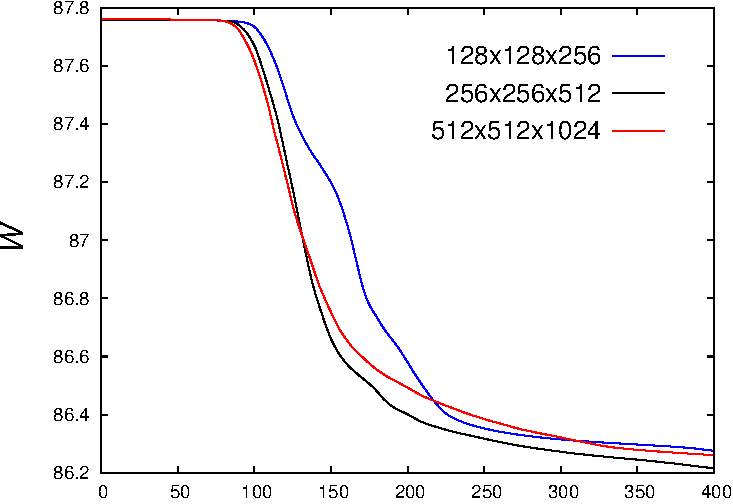
\includegraphics[scale=0.5]{./gnuplot/en_w}
  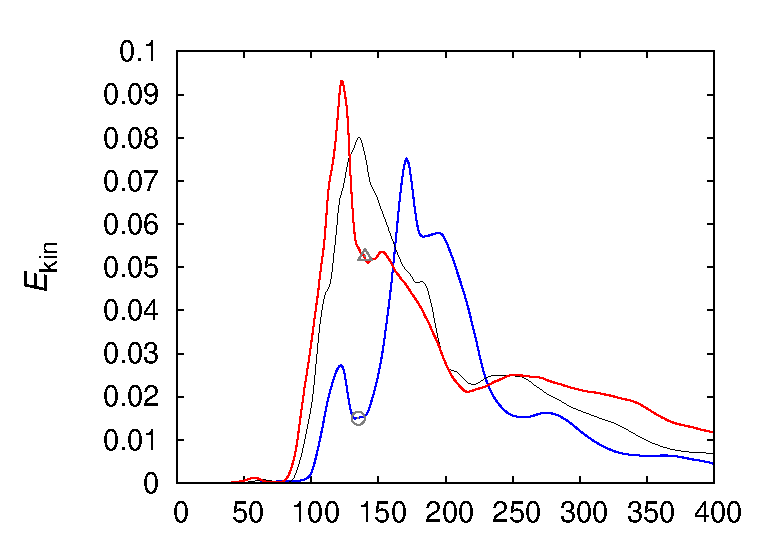
\includegraphics[scale=0.5]{./gnuplot/en_kin}\\
  \vspace{10pt}
  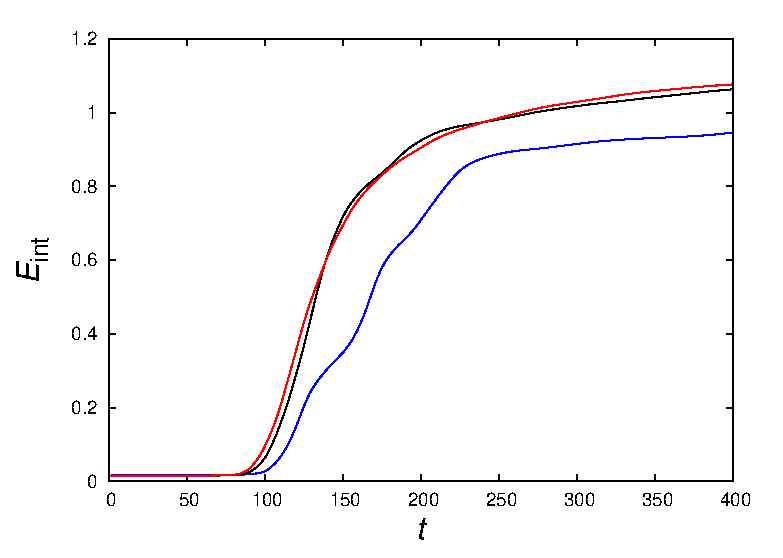
\includegraphics[scale=0.5]{./gnuplot/en_int}
  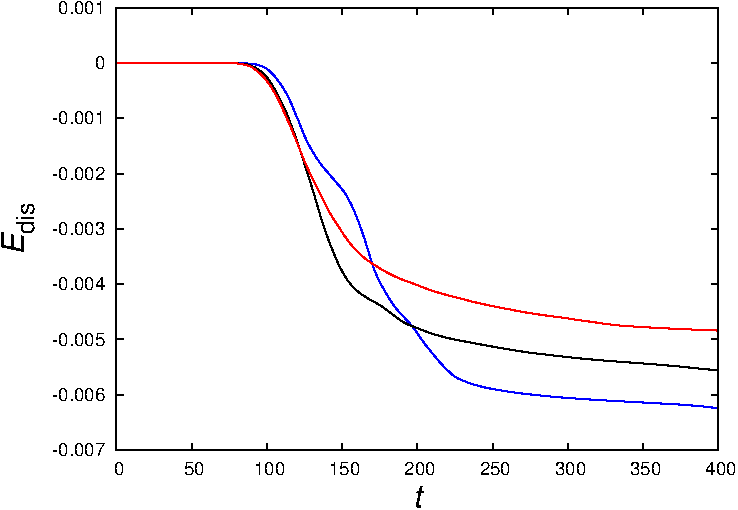
\includegraphics[scale=0.5]{./gnuplot/en_dis}
  \caption{\small{The magnetic energy (top left), kinetic energy (top right), internal energy (bottom left), and numerical dissipation (bottom right) at resolutions of $128^{\,2} \times 256$ (blue), $256^{\,2} \times 512$ (black) and $512^{\,2} \times 1024$ (red).}}
  \label{en}
\end{figure}
There is little difference in the amount of energy released by the magnetic field, which indicates that the energy release is entirely defined by the nature of the unstable equilibrium. The two most highly resolved simulations achieve instability about $20\,t_{\mathrm{A}}$ earlier than the low resolution case. Numerical dissipation ($E_{\mathrm{dis}}\,{=}\,E_{\mathrm{tot}}(t)/E_{\mathrm{tot}}(0)\,-\,1$, where $E_{\mathrm{tot}}\,=\,W\,+\,E_{\mathrm{kin}}\,+\,E_{\mathrm{int}}$) is lowest for the highest resolution case and is just under $0.5\%$. The amount of Ohmic heating reduces markedly with increasing resolution. Figure \ref{ht_visc_ohmic} (left) shows the ratio of the total shock heating to the total Ohmic heating as a function of time. As $\delta x$ is decreased, the critical current threshold rises (see equation \ref{eqn_critical_current5}) and the opportunities for anomalous resistivity are much reduced. This relationship outweighs the fact that better resolved currents are typically higher (Figure \ref{ht_visc_ohmic}, right).
\begin{figure}[h!]
  \center  
  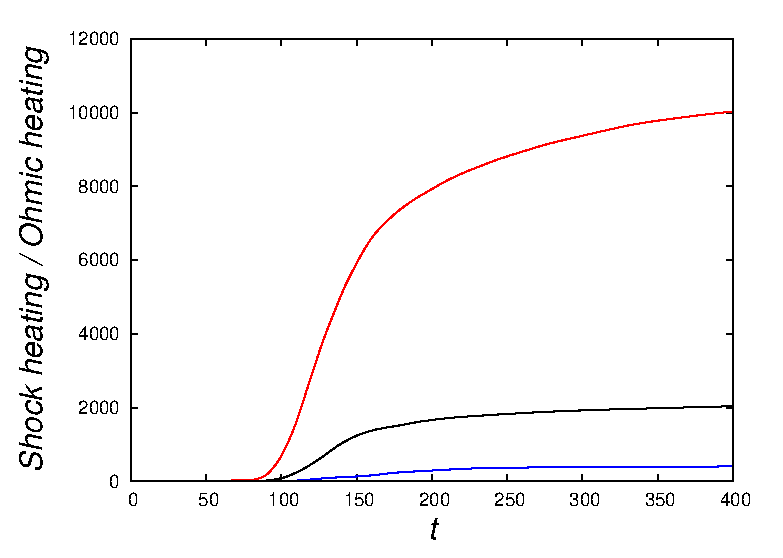
\includegraphics[scale=0.5]{./gnuplot/ht_visc_ohmic}
  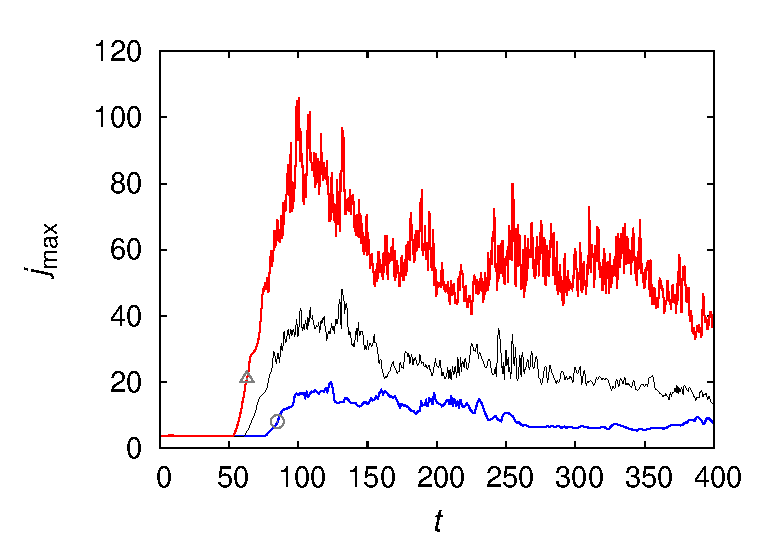
\includegraphics[scale=0.5]{./gnuplot/j_max}
  \caption{\small{The ratio of shock heating to Ohmic heating (left) and maximum current density (right) at resolutions of $128^{\,2} \times 256$ (blue), $256^{\,2} \times 512$ (black) and $512^{\,2} \times 1024$ (red).}}
  \label{ht_visc_ohmic}
\end{figure}

What is significant about these results is that our attempts to maximise Ohmic dissipation by using a locally-defined current threshold have instead confirmed the dominance of shock heating. Between the $128^{\,2} \times 256$ and $256^{\,2} \times 512$ simulations, the shock heating increases by about $10\%$; however, a further increase in spatial resolution leaves the level of shock heating more or less unchanged. The gradients in kinetic energy that LARE3D interprets as shock heating are not an artefact of inadequate resolution. Henceforth, figures and plots will be taken from the $256^{\,2} \times 512$ simulation.

\subsection{Shock heating}
\label{sec_NumericalResults_ShockHeating}
It is instructive to break down the shock heating into its constituent tensor components, where each component is identified by $\varepsilon_{ij}\,-\,(1/3)\,\delta_{ij}\,\nabla\cdot\vec{v}\,$ (equation \ref{eqn_lare_shock_viscosity_tensor}) --- the possible $ij$ pairs are $xy$, $xx$, $yy$, $xz$, $yz$ and $zz$ (Figure \ref{ht_visc_comp}).
\begin{figure}[h!]
  \center  
  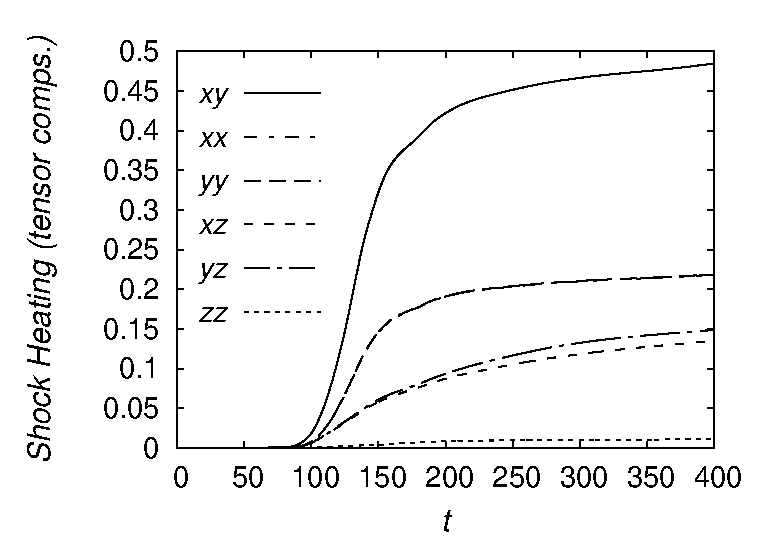
\includegraphics[scale=0.55]{./gnuplot/256x256x512/ht_visc_comp}
  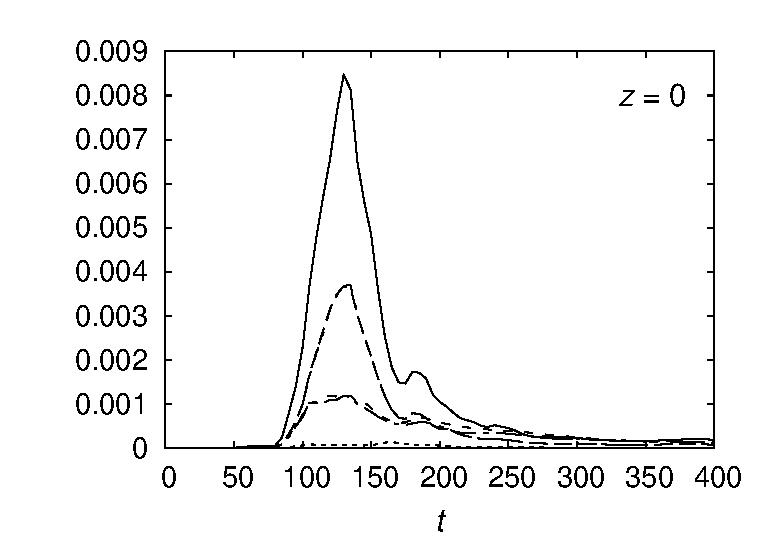
\includegraphics[scale=0.55]{./gnuplot/256x256x512/ht_visc_comp_apex}
  \caption{\small{The shock heating tensor components for the whole simulation domain (left) and for the loop apex only (right). The $xx$ and $yy$ components follow each other and for the left plot have a final value of 0.2.}}
  \label{ht_visc_comp}
  \vspace{-10pt}
\end{figure}
 The shock heating is mostly due to the spatial variation of the $x$ and $y$ components of velocity in the azimuthal plane. Roughly one quarter of the heating is due to changes in $v_x$ and $v_y$ with respect to $z$, and very little is contributed by the $zz$ component. 

Figure \ref{xy_visc_map} shows the distribution of shock heating at the beginning of the instability ($t\,{=}\,95\,t_{\mathrm{A}}$).
\begin{figure}[h!]
  \center  
  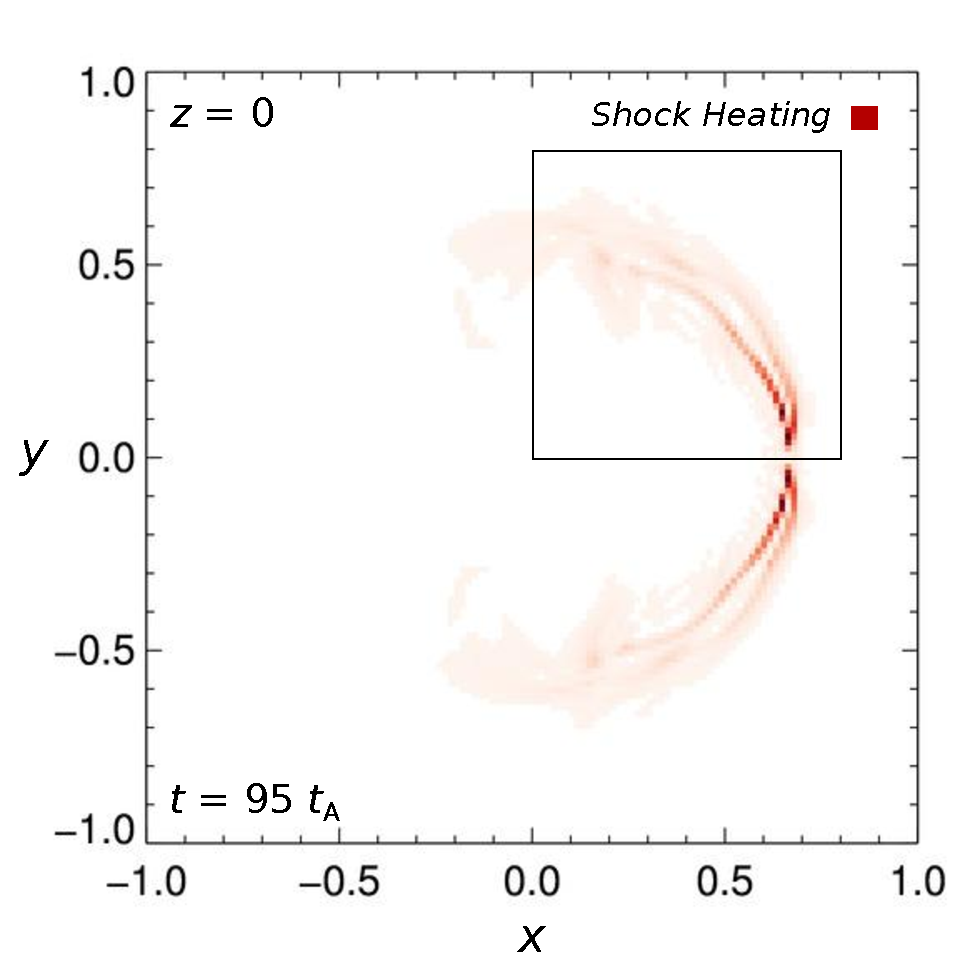
\includegraphics[scale=0.415]{./inkscape/256x256x512/xy_visc_sca}
  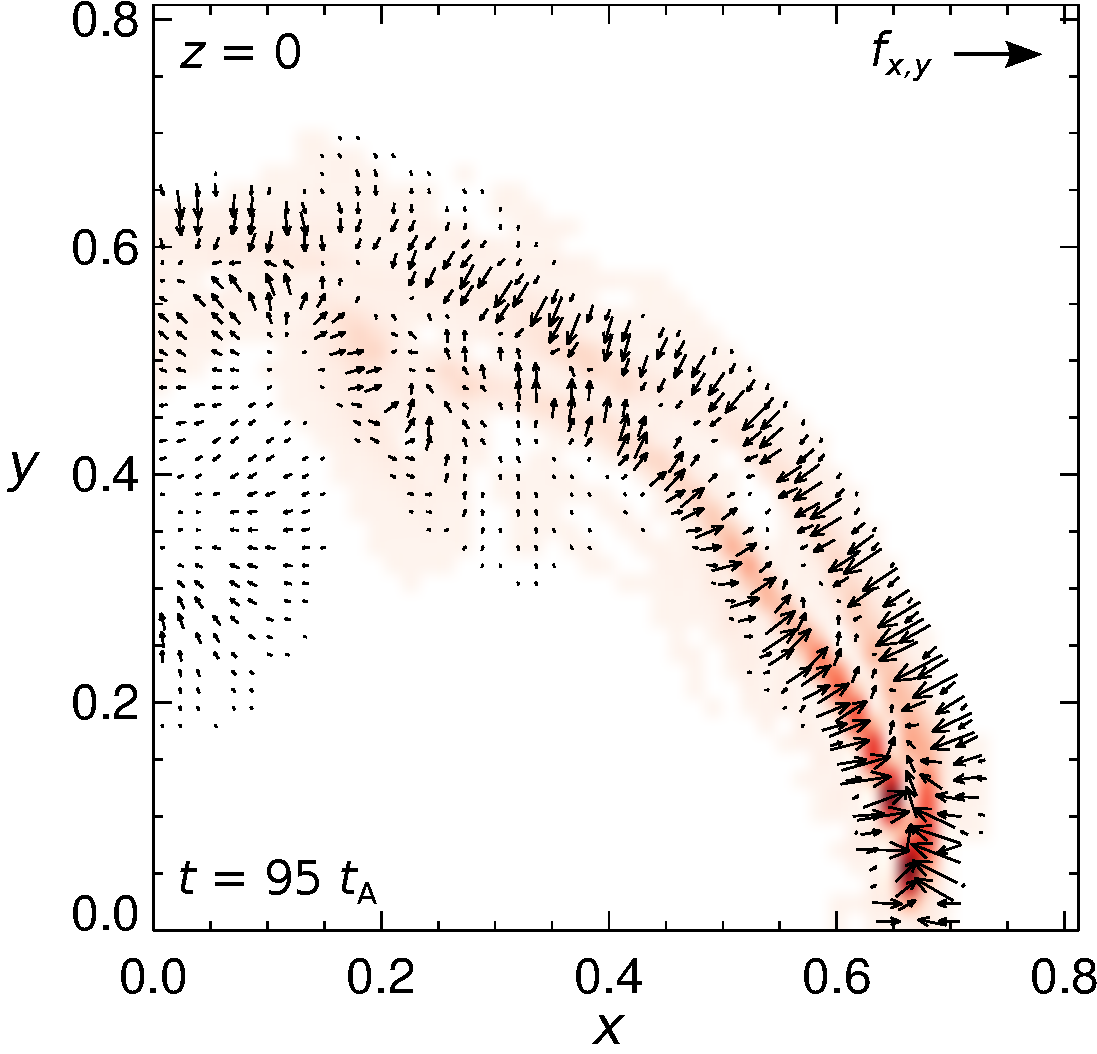
\includegraphics[scale=0.35]{./inkscape/256x256x512/visc_sca_rf_vec}
  \caption{\small{\textbf{Left}, the shock heating over the $x$-$y$ plane at $t\,{=}\,95\,t_{\mathrm{A}}$ and $z\,{=}\,0$. \textbf{Right}, part of the top right quadrant of the midplane with the in-plane Lorentz forces superimposed as arrows.}}
  \label{xy_visc_map}
  \vspace{-10pt}
\end{figure}
The shock heating is concentrated where the loop has kinked outwards against the external potential field. The curved bands of Figure \ref{xy_visc_map}, which are indicative of Petschek reconnection, curve inwards towards the loop axis as one increases or decreases the $z$ coordinate. The left plot of Figure \ref{xy_visc_map} is symmetrical about $y\,{=}\,0$; thus the top right quadrant is expanded so as to follow the shock heating in more detail. There are in fact two thin bands of shock heating that appear to trace the azimuthal magnetic field --- between the two curved bands the shock heating is minimal. At this time, there are no super-critical currents around the midplane: Ohmic dissipation is therefore non-existent within Figure \ref{xy_visc_map}. 

If the dissipation of magnetic energy is responsible for the rise in shock heating then these two events must be connected by the Lorentz force. At every time step the Lorentz term is calculated and used to update the velocity via the equation of motion. Shock heating might occur if such updates create sharp spatial gradients of velocity. Figure \ref{xy_visc_map} (right) shows a strong correlation between the Lorentz vectors (projected in the $x$-$y$ plane) and the areas of strongest shock heating. The inner band of heating appears to be caused by Lorentz forces that are generally acting in a radially outward direction, whereas a radially inward force coincides with the outer band. In between the two bands the Lorentz force is minimal and so is the shock heating. The reason for the shock heating \textit{gap} must relate to the lack of a Lorentz force. Within the gap, current and magnetic field magnitudes are non-zero; hence, the only way for the Lorentz force (and the shock heating) to become negligible is for the current and magnetic field vectors to become aligned. 

\begin{figure}[h!]
  \center  
  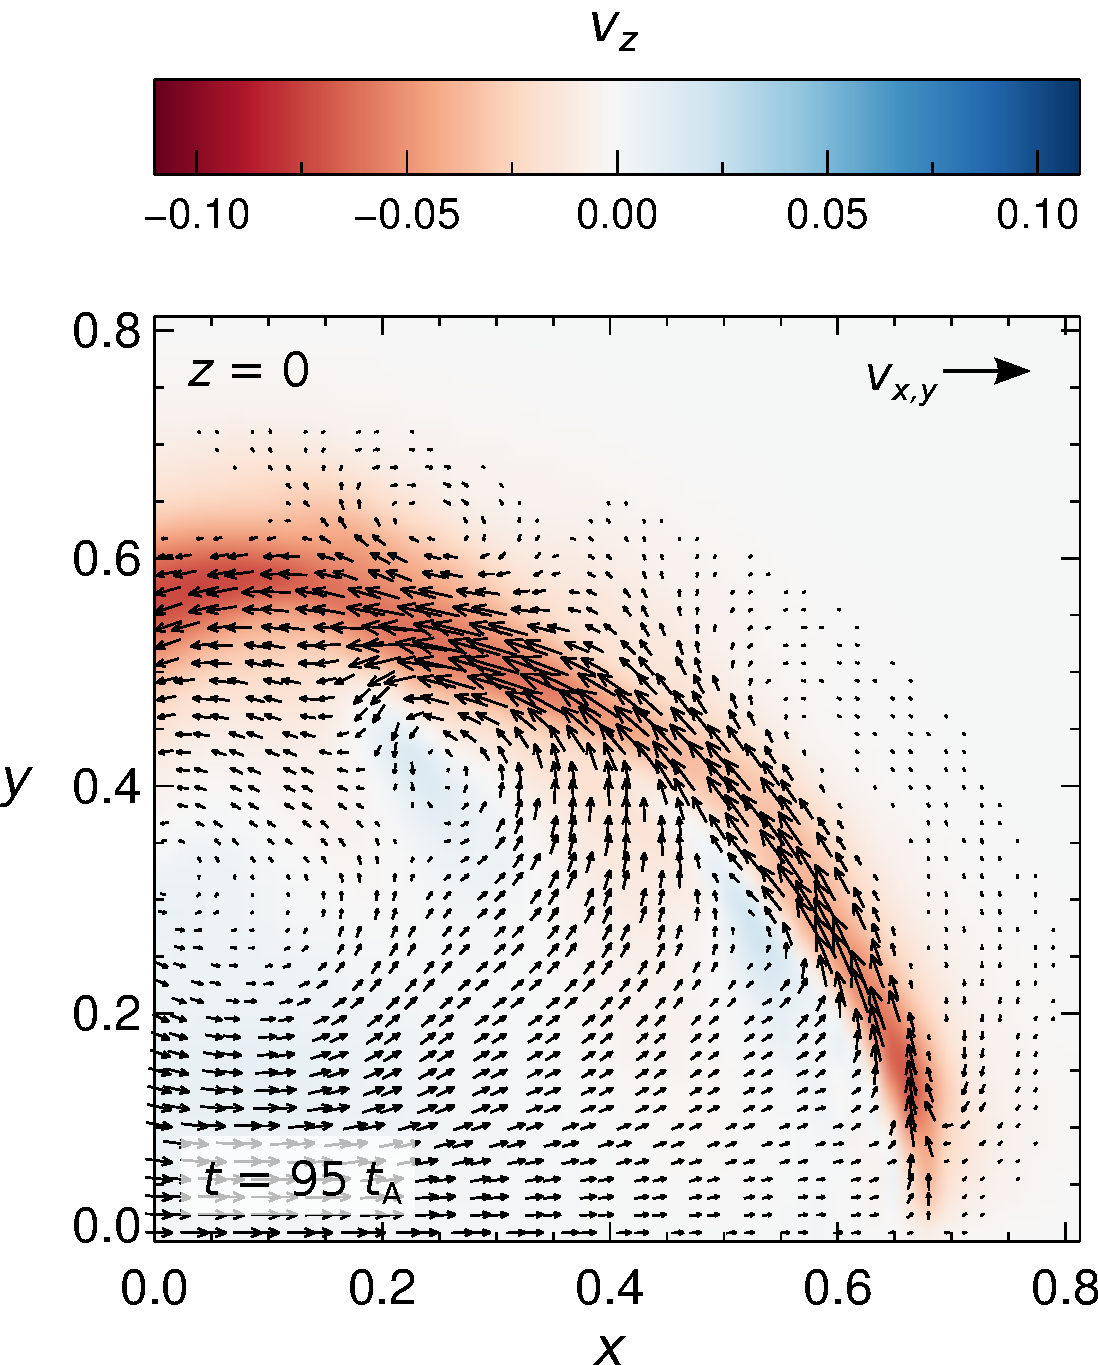
\includegraphics[scale=0.35]{./inkscape/256x256x512/vz_sca_v_vec}
  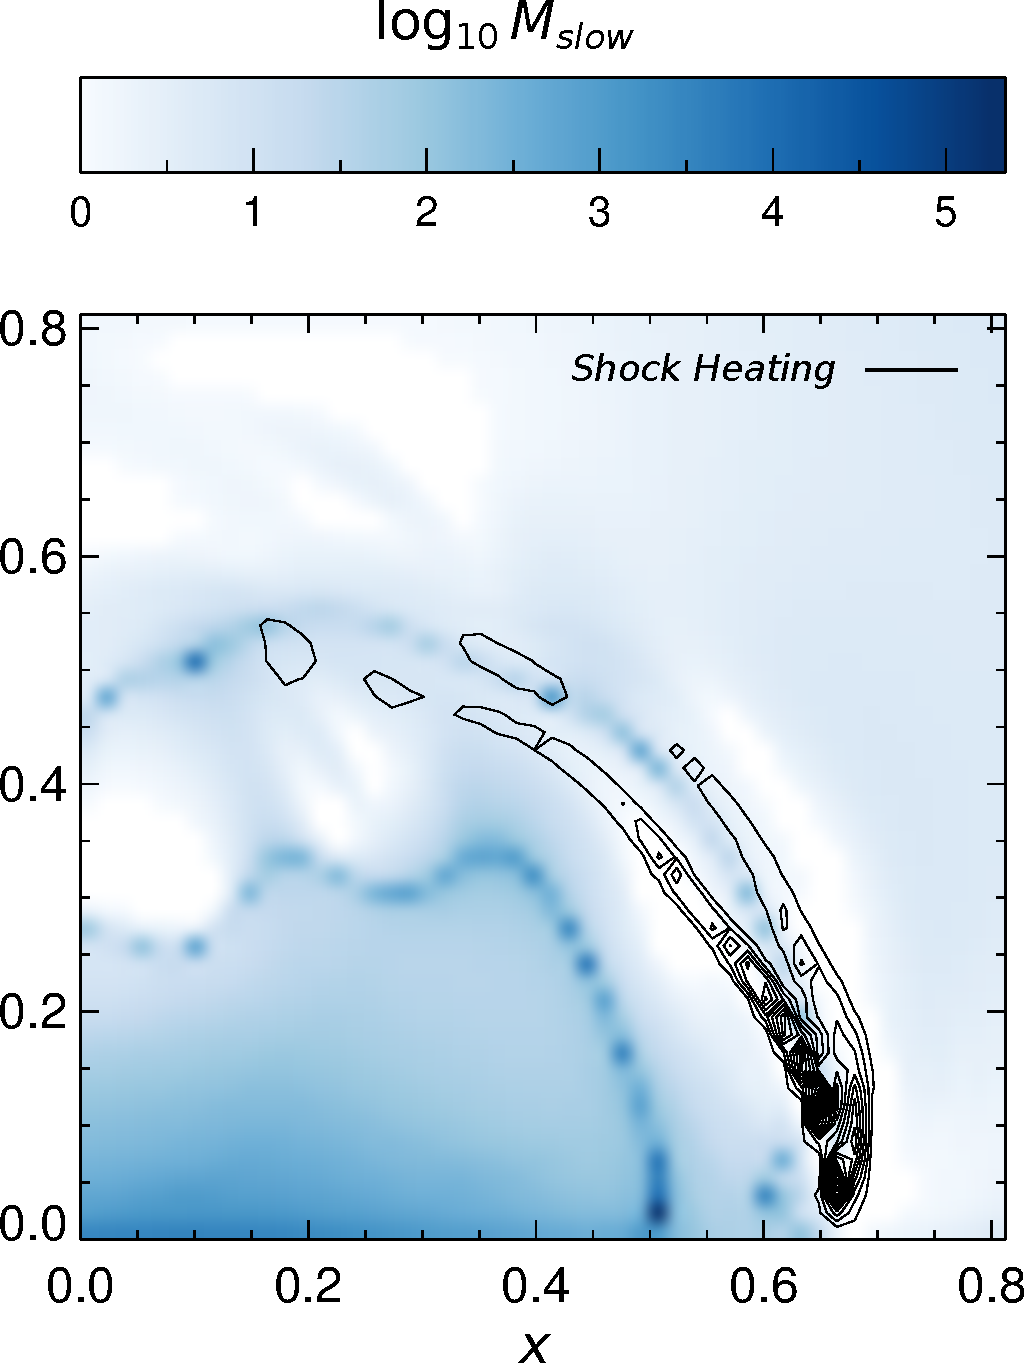
\includegraphics[scale=0.35]{./inkscape/256x256x512/slow_mach_sca_visc_con}
  \caption{\small{\textbf{Left}, coloured contours of $v_{z}$ over a subsection of the midplane with inplane velocity vectors, where $\mathrm{MAX}(|v_{x,y}|)\,{=}\,0.11$. \textbf{Right}, the base 10 logarithm of the slow mode Mach number over the same region with contours of shock heating.}}
  \label{v_and_slow_mach}
  \vspace{-10pt}
\end{figure}

The Lorentz forces are dominated by the $x$ and $y$ components: moreover, it is striking to see two sets of anti-parallel Lorentz vectors (corresponding to the two bands of shock heating), see Figure \ref{xy_visc_map} (right). If these results are compatible with Petschek reconnection there should be two shock front normals pointing outwards from the gap, which outlines the current sheet thickness. The sheet width would have a component out of the plane (parallel to the $z$-axis). Figure \ref{v_and_slow_mach} (left) allows us to examine the plasma flow pattern. Note, the magnitude of the inplane velocity is given by the length of the arrow, and the longest arrows correspond to a velocity of $0.11$, the limit of the $v_z$ colour bar. Thus, at $x\,{=}\,y\,{=}\,0.5$ there is a plasma flow where the azimuthal and axial components are roughly equal ($v_z\,{\approx}\,0.7$), and so, Figures \ref{xy_visc_map} and \ref{v_and_slow_mach} present us with an oblique line of sight into a plasma outflow region. The slow mode speed varies according to local conditions, since it is dependent on temperature, density, field strength and velocity, all of which are non-uniform.
For this reason we plot the logarithm of the slow mode speed Mach number (Figure \ref{v_and_slow_mach}, right) in order to confirm the presence of supersonic flows. Notice also that the shock heating contours mostly surround regions coloured white: the slowing of shocked plasma to subsonic speeds correctly coincides with regions of heating.

Further insight is gained by comparing the distribution of Lorentz vectors with two other properties (Figure \ref{plasmab_and_jz}), specifically, plasma-$\beta$ (left) and the axial current (right). Inside the shock heating gap, the plasma density and field strength are reduced, whereas temperature is increased; the plasma-$\beta$ is therefore enhanced in this location.
\begin{figure}[h!]
  \center  
  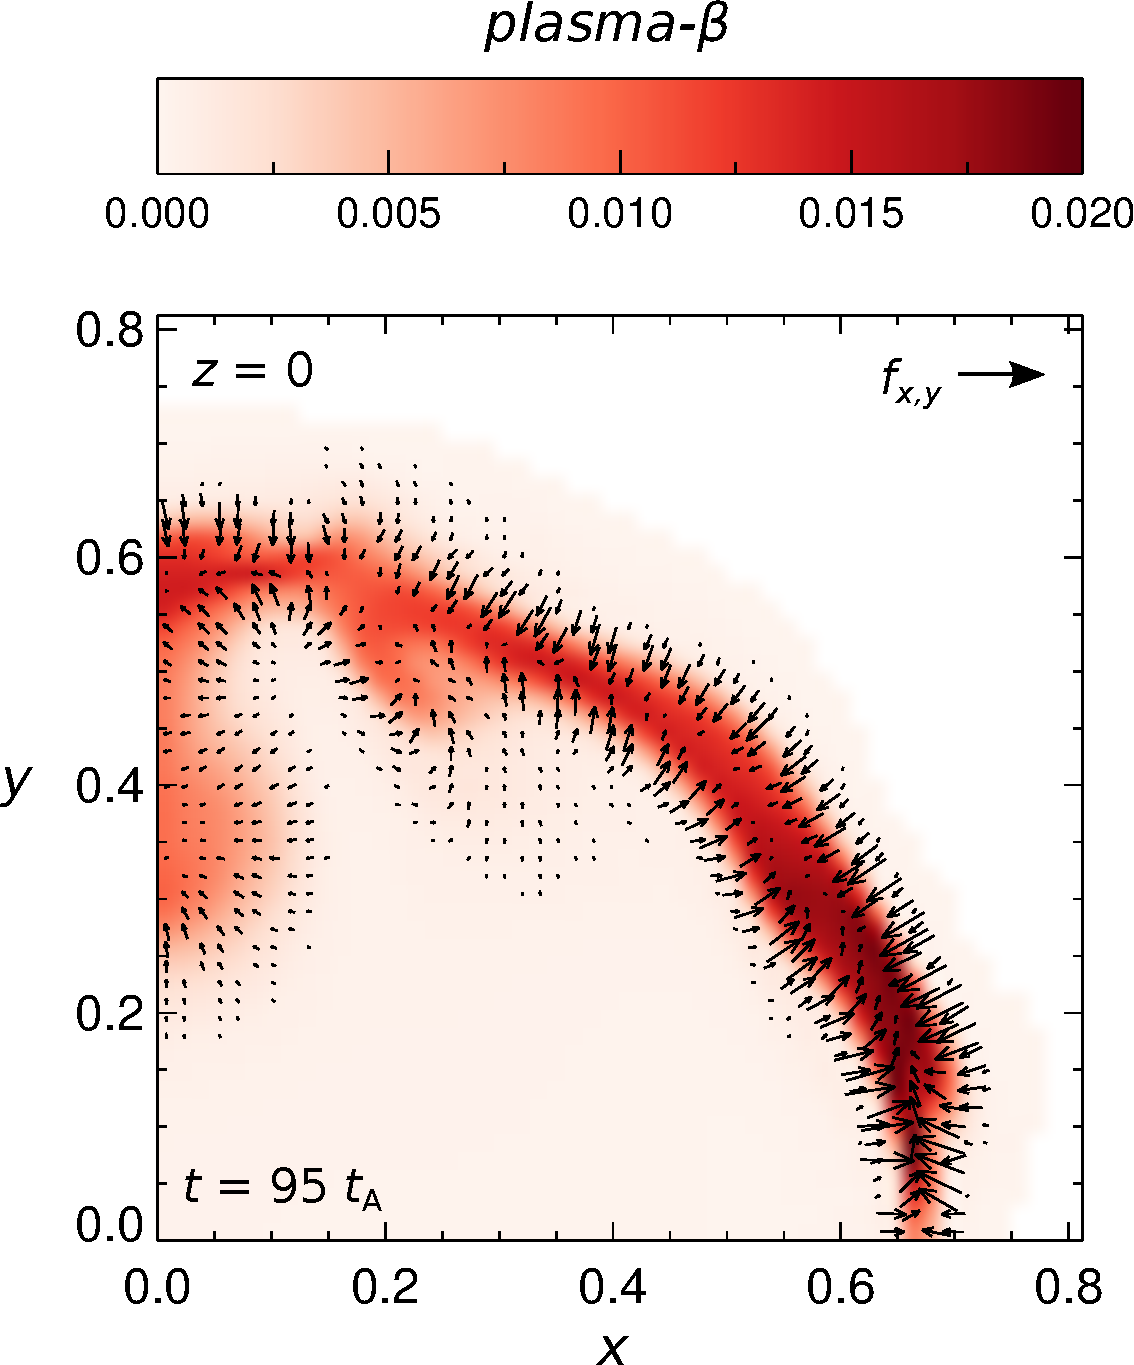
\includegraphics[scale=0.35]{./inkscape/256x256x512/plasmab_sca_rf_vec}
  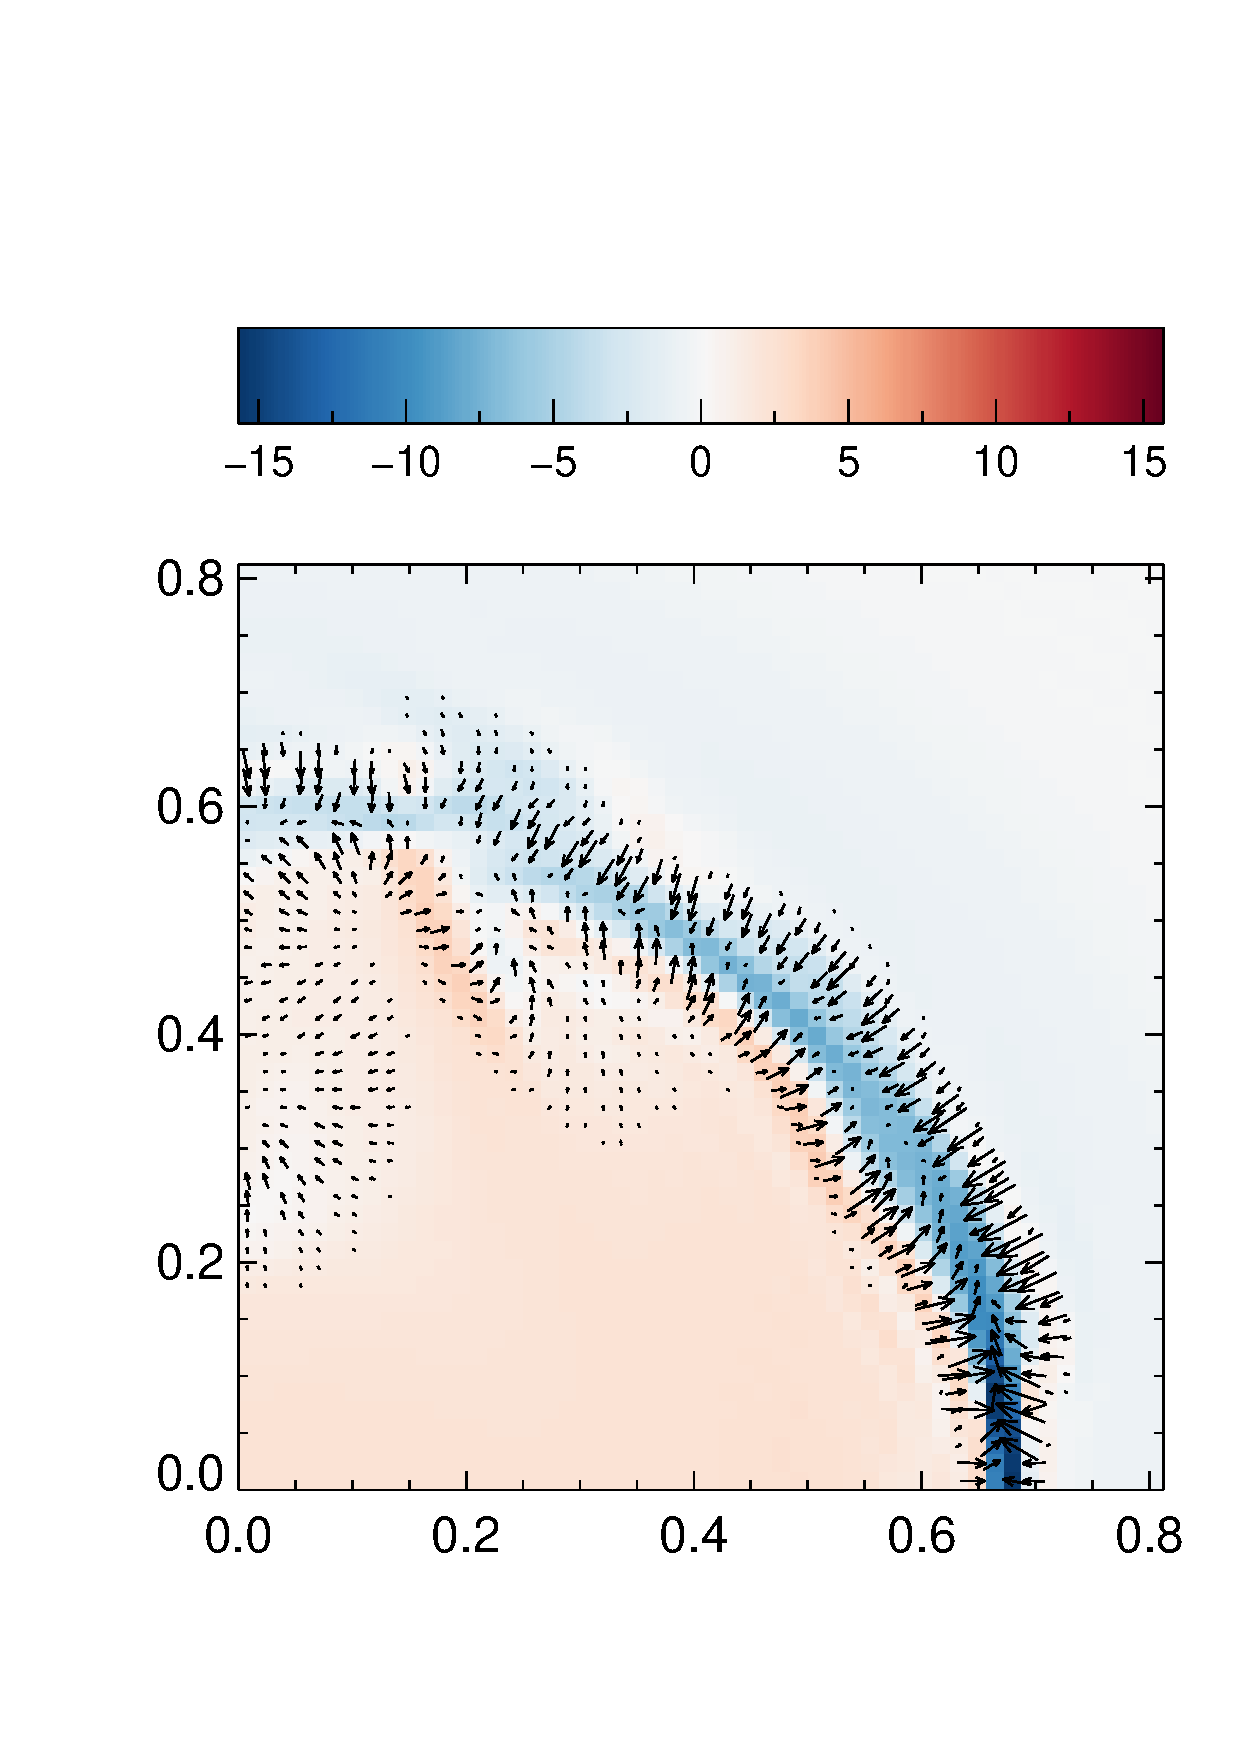
\includegraphics[scale=0.35]{./inkscape/256x256x512/jz_sca_rf_vec}
  \caption{\small{\textbf{Left}, coloured contours of plasma-$\beta$ over a subsection of the midplane with inplane Lorentz vectors. \textbf{Right}, the axial current ($j_z$) over the same region.}}
  \label{plasmab_and_jz}
  \vspace{-10pt}
\end{figure}
Turning our attention to the right plot, the inner band of shock heating is just outside (radially speaking) a similarly curved band of positive axial current, and the outer band of shock heating coincides with the inward pointing Lorentz vectors, which have been generated by negative axial current. Where the axial current is strongest (i.e., most negative) there are no significant Lorentz vectors, since in that region $\vec{j}\times\vec{B}\,\,{\approx}\,\,0$. At the start of the simulation, there is a positive current flowing at the centre of the midplane, surrounded by a ring of weaker negative current, in accordance with the initial $B_{\theta}$ field. When the instability develops, the kinking motion compresses any plasma in its path and thereby enhances the magnitudes of the axial currents. Figure \ref{plasmab_and_jz} (right) reveals that the outwardly radial direction described by the kinking begins just inside the region of positive current. Hence, some positive $j_z$ is amplified, creating the outward pointing Lorentz vectors: however, the larger region of negative axial current produces a stronger $j_z$, which creates the opposing Lorentz forces.
\begin{figure}[h!]
  \center  
  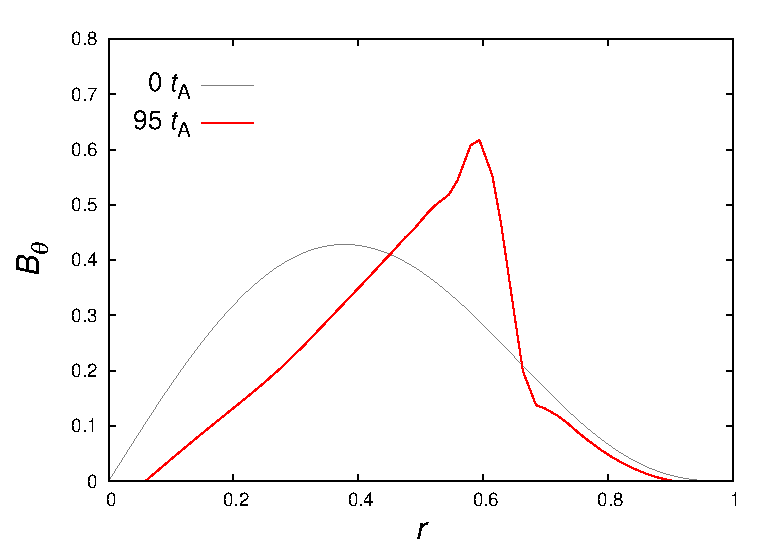
\includegraphics[scale=0.52]{./gnuplot/256x256x512/btheta_r_19}
  \hspace{5pt}
  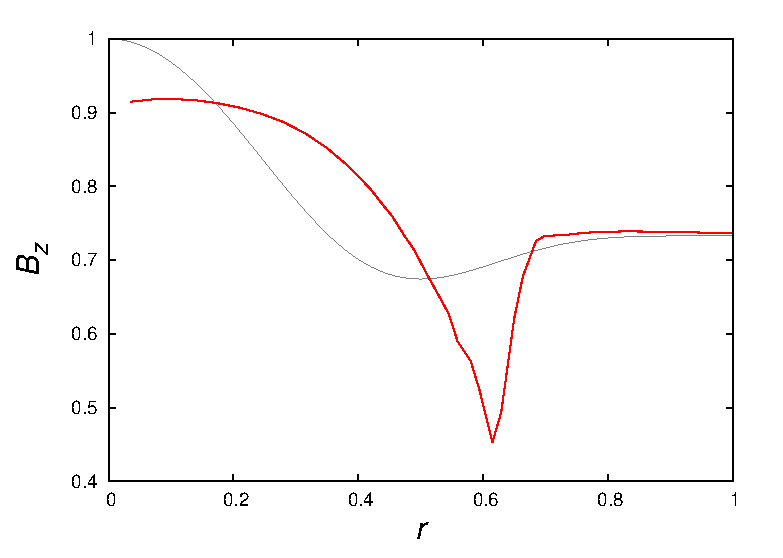
\includegraphics[scale=0.52]{./gnuplot/256x256x512/bz_r_19}
  \caption{\small{Plots of $B_{\theta}(r)$ (left) and $B_{z}(r)$ across the midplane at $\theta\,{=}\,27^{\circ}$ for time $t\,{=}\,0$ (grey) and $t\,{=}\,95\,t_{\mathrm{A}}$ (red).}}
  \label{b_rad}
  \vspace{-10pt}
\end{figure}
Of course, these changes in the axial current profile also alter the azimuthal field, see the red plots of Figure \ref{b_rad}. As the kink instability gets under way, magnetic energy is converted into kinetic; this amplifies the kinking, giving rise to strong helical currents, which create a locally enhanced azimuthal field. Magnetic flux is conserved and so moves with the plasma; hence an enhanced azimuthal field must correspond to a diminished axial field - Figure \ref{b_rad} shows this to be the case.

\subsection{Global evolution}
\label{sec_NumericalResults_GlobalEvolution}

The plots so far have all been taken at the midplane ($z\,{=}\,0$). For this reason, the final two figures are intended to give a sense of the global changes in plasma temperature and magnetic field. 
\begin{figure}[h!]
  \center  
  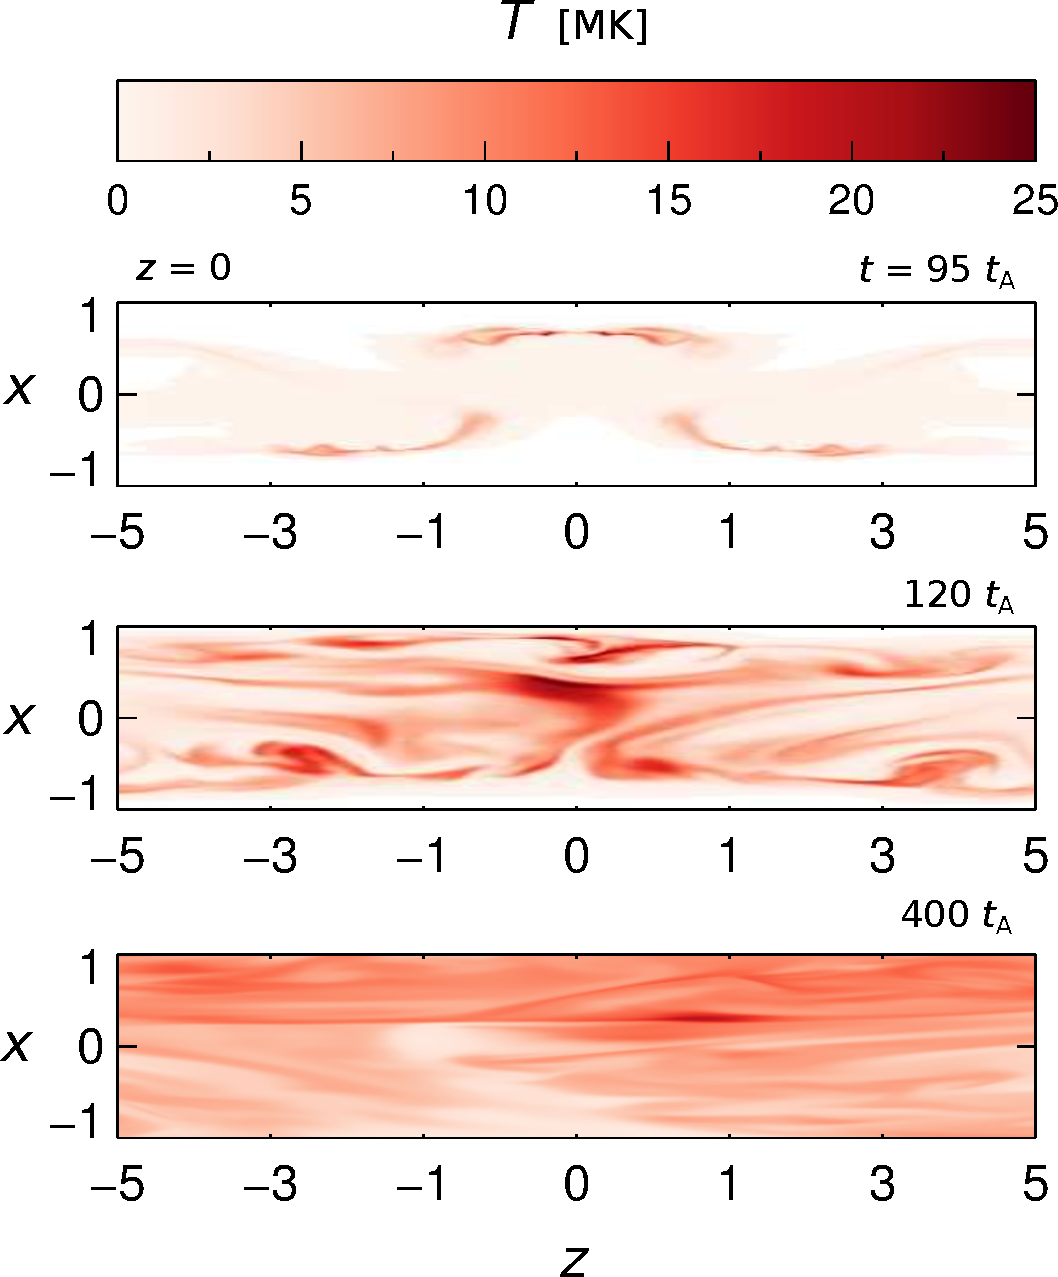
\includegraphics[scale=0.38]{./inkscape/256x256x512/xz_temp_sca}
  \caption{\small{Plasma temperature over the $x$-$z$ plane at $y\,{=}\,0$ for three times, at the start of the kink instability (top), during the instability (middle) and at the end of the simulation (bottom).}}
  \label{xz_temp}
  \vspace{-10pt}
\end{figure}
Figure \ref{xz_temp} shows cross sections of the temperature (scaled acccording to the values given in \mbox{Section \ref{sec_NumericalCode}}) at three times during the simulation. We find that the situation seen at the midplane is also applicable to other $z$-coordinates: at $t\,{=}\,95\,t_{\mathrm{A}}$ (the start of the instability), slow mode shocks are creating high temperatures at two other sections along the loop, near the $x\,{=}\,-0.5$ line. The hot (red) areas are where the loop is kinking outwards against the outer potential field. Subsequently, the plasma becomes more turbulent, before starting a slow relaxation to a uniform temperature.

The field configuration undergoes similar changes to those seen in other simulations of kink unstable loops. At instability onset, the magnetic field starts to undergo a helical kink; the following turbulent phase results in a loss of azimuthal field ($B_{x,y}$), which leaves a predominantly axial field by the end of the simulation (Figure \ref{bfield_voheat}).
\begin{figure}[h!]
  \center  
  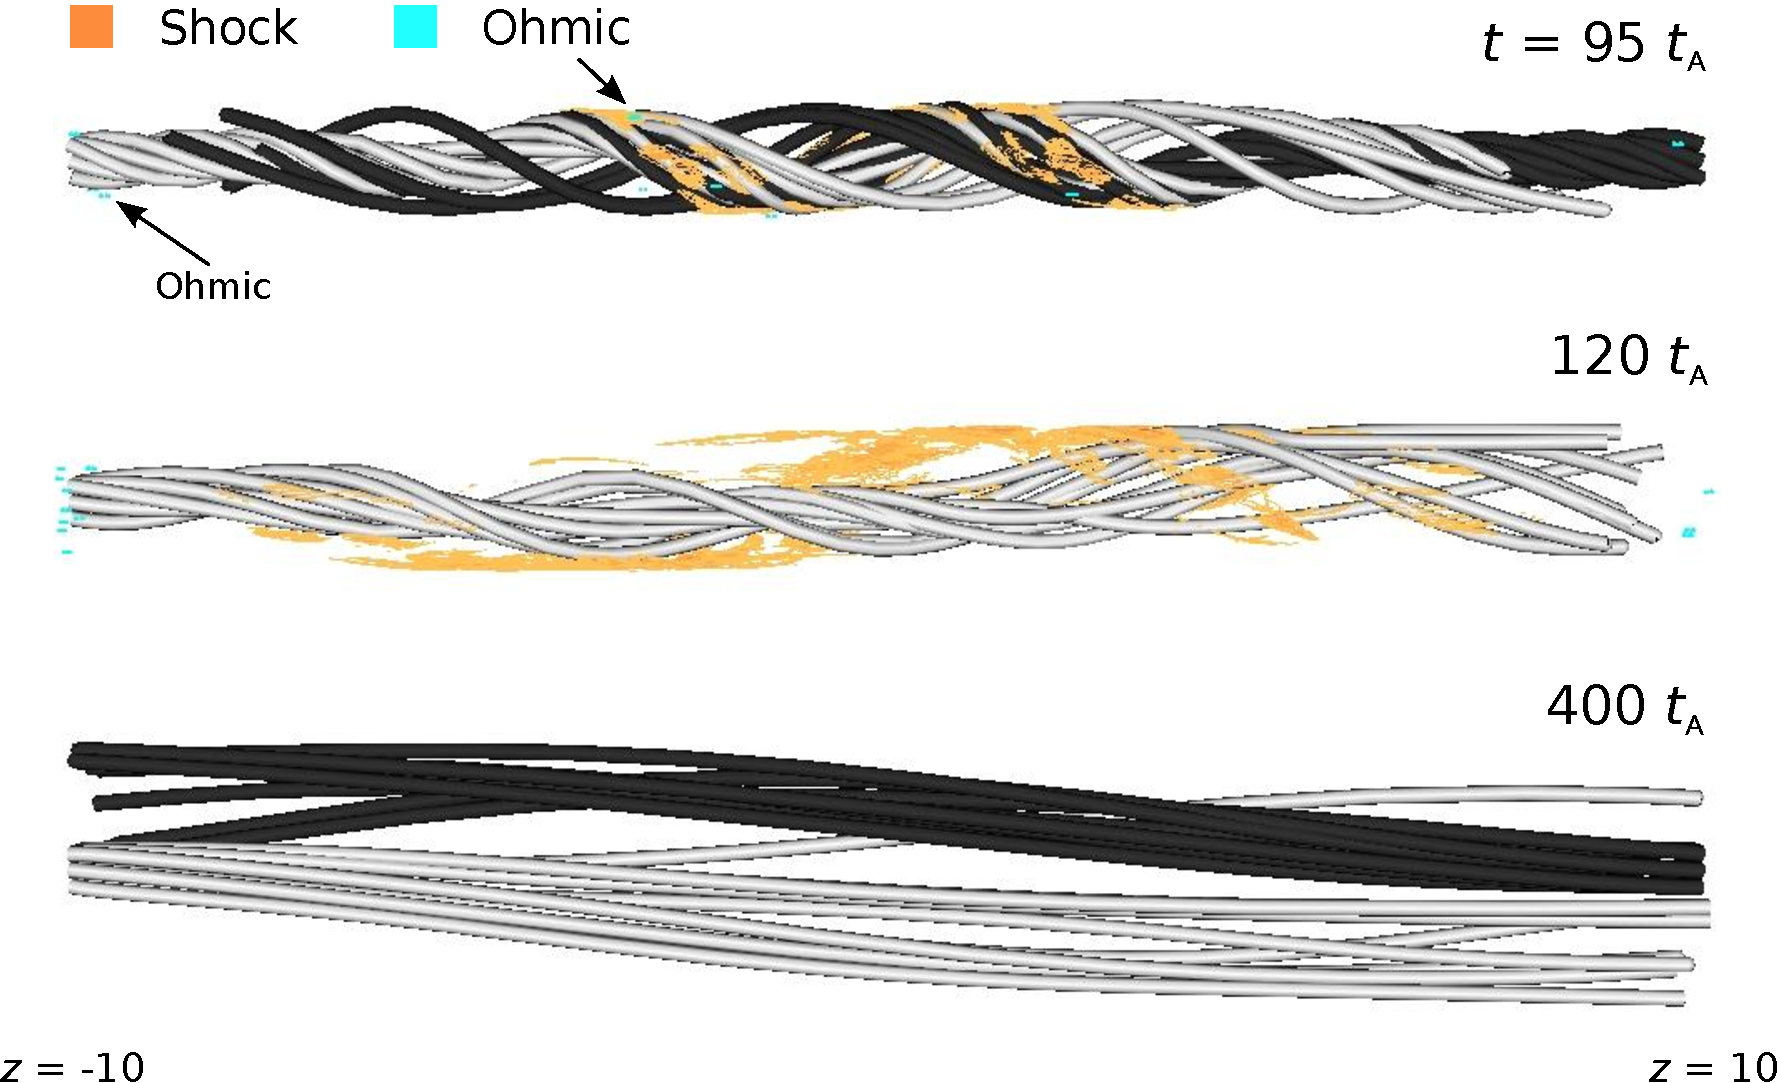
\includegraphics[scale=0.4]{./inkscape/256x256x512/bfield_voheat}
  \caption{\small{Magnetic field lines originating from the left footpoint (light grey) and from the right footpoint (dark grey) are shown for three times, $t\,{=}\,95\,t_{\mathrm{A}}$ (top), $120\,t_{\mathrm{A}}$ (middle) and $400\,t_{\mathrm{A}}$ (bottom). The plots are shown with isosurfaces of shock heating (orange) and Ohmic heating (cyan). Dark grey field lines, originating from $z\,{=}\,10$, have been removed from the middle plot for clarity.}}
  \label{bfield_voheat}
  \vspace{-10pt}
\end{figure}
It is noticeable that the kinking is more radially confined compared to past work, see Figure 6 of Bareford et al. [17] and Figure 10 of \mbox{Hood et al. [13]}. We attribute this to two aspects of the initial equilibrium, a smooth $\alpha$-profile and zero net current, that force $B_{\theta}$ to have a maximum at $r\,{\approx}\,0.4$. Although the cited work also features loops of zero net current, $\alpha (r)$ has a piecewise-constant profile, resulting in high axial currents near the loop boundary at $r\,{=}\,1$. Another important difference is in the way Ohmic heating is handled. Bareford et al. [17] found that regions of Ohmic heating appeared more or less at the same locations (and times) as shock heating, although the latter was far stronger than the former. By contrast, the use of a variable critical current employed here produces small pockets of Ohmic heating scattered near the footpoints and around the midplane. In Figure \ref{bfield_voheat}, we use arrows to point out two of these pockets. Ohmic heating ceases completely after $t\,{=}\,170\,t_{\mathrm{A}}$, and at the end of the simulation, shock heating is an order of magnitude lower than what it was at $120\,t_{\mathrm{A}}$. 

\section{Summary and conclusions}
\label{sec_summary_conclusions}

We have taken an initial field configuration, representing a straightened coronal loop, and induced an instability with the intention of investigating how the magnetic energy released is converted into heat. The ideal kink instability converts mainly azimuthal field (i.e., $B_x$ and $B_y$) into Lorentz forces, which increases kinetic energy, thereby amplifying the kink. The resulting compression of plasma generates high (compared to the initial state) helical currents; this increases the Lorentz forces further, which feeds back to the velocity and ultimately generates heating through shock viscosity. In other words, sharp gradients in velocity (created by Lorentz forces), shear and compress local grid cells. The entropy production implied by these sudden changes in velocity are captured by shock viscosity. The subsequent heating causes a drop in velocity via the viscous term ($\nabla\cdot\vec{\sigma}$) in the equation of motion. This velocity reduction then leads to field dissipation when those same velocities are used to remap field components back to the Eulerian grid via the induction equation. It is at this stage that numerical dissipation occurs, since the use of van Leer gradient limiters during the remap, exaggerates the reduction in magnetic field strength. This is confirmed by the energy plots (Figure \ref{en}) --- too much magnetic energy is dissipated compared to the level of shock heating. Interestingly, this numerical dissipation is much reduced when the coronal loop is only marginally unstable (i.e., $\lambda\,{=}\ 1.62$), then the dissipation is only $0.36\%$ of the initial total energy for a spatial resolution of $256^2\times512$.

It seems that employing a more realistic scheme as regards the application of anomalous resistivity (Section 3 \ref{sec_NumericalCode_CriticalCurrentDensity}) reduces severely the opportunities for Ohmic dissipation (Figure \ref{ht_visc_ohmic}). In the simulations presented here, it is the shock heating that causes the magnetic field to lose energy and relax to a lower energy state. In theory, if there were no form of heating, energy would forever move back and forth between kinetic and magnetic. Instead, the shock heating weakens axial current flow and reduces $B_x$ and $B_y$; in other words, the kinetic energy causing the shock is not simply returned to the field.

Figures \ref{xy_visc_map}-\ref{plasmab_and_jz} demonstrate that the plasma dynamics causing the heating are consistent with Petschek reconnection and slow mode shocks. The advantage of this dissipation mechanism is that it can operate within a collisonless regime such as the corona. One key assumption made here, is that the net result of photospheric convective motions \textit{twist} the magnetic fields that reach into the corona. Over time, these fields would become susceptible to the kink instabitiy, which, as this work shows, is a sufficient condition for coronal heating via slow mode shocks. We expect these findings will apply to more realistic loop models; ones that feature thermal condition, atmospheric stratification and loop curvature ([27,28,30]). Shock heating may also occur for other types of instability (e.g, torus or ballooning), especially it it causes a coronal loop to rapidly expand into an overlying field. 


\section*{Acknowledgments}

We thank the referees for their helpful comments and gratefully acknowledge the compute time (STFC funded) granted for the DiRAC and UKMHD facilities. The simulations were run on the UK MHD cluster at St Andrews University and on the COSMA Data Centric system at Durham University. The latter facility is operated by the Institute for Computational Cosmology on behalf of the STFC DiRAC HPC Facility (www.dirac.ac.uk), and the computer hardware was funded by a BIS National E-infrastructure capital grant ST/K00042X/1, DiRAC Operations grant ST/K003267/1 and Durham University --- DiRAC is part of the National E-Infrastructure.

\begin{thebibliography}{9}
\bibitem{1} Hood AW. 1992. \textit{Plasma Physics and Controlled Fusion} \textbf{34}
\bibitem{2} Browning PK, Van der Linden RAM. 2003. \textit{A\&A} \textbf{400}
\bibitem{3} Haynes M, Arber TD. 2007. \textit{A\&A} \textbf{467}
\bibitem{4} Srivastava AK, Zaqarashvili TV, Kumar P, Khodachenko ML. 2010. \textit{ApJ} \textbf{715}
\bibitem{5} Hood AW, Priest ER. 1979. \textit{Sol. Phys.} \textbf{64}
\bibitem{6} Baty H, Heyvaerts J. 1996. \textit{A\&A} \textbf{308}
\bibitem{7} Velli M, Lionello R, Einaudi G. 1997. \textit{Sol. Phys.} \textbf{172}
\bibitem{8} Arber TD, Longbottom AW, Van der Linden RAM. 1999. Title. \textit{ApJ} \textbf{517}
\bibitem{9} Baty H. 2000. \textit{A\&A} \textbf{353}
\bibitem{10} Galsgaard K, Nordlund \AA. 1996. \textit{J. Geophys. Res.} \textbf{101}
\bibitem{11} Gudiksen BV, Nordlund \AA. 2005. \textit{ApJ} \textbf{618}
\bibitem{12} Browning PK, Gerrard C, Hood AW, Kevis R, Van der Linden RAM. 2008. \textit{A\&A} \textbf{485}
\bibitem{13} Hood AW, Browning PK, Van der Linden RAM. 2009. \textit{A\&A} \textbf{506}
\bibitem{14} Bourdin PA, Bingert S, Peter H. 2013. \textit{A\&A} \textbf{555}
\bibitem{15} Rappazzo AF, Velli M, Einaudi G. 2013. \textit{ApJ} \textbf{771}
\bibitem{16} Chen F, Peter H, Bingert S, Cheung MCM. 2014. \textit{ApJ} \textbf{564}
\bibitem{17} Bareford MR, Hood AW, Browning PK. 2013. \textit{A\&A} \textbf{550}
\bibitem{18} Priest ER. 1987 \textit{Solar Magnetohydrodynamics}. D. Reidel Publishing Company (Dordrecht, The Netherlands)
\bibitem{19} Petschek HE. 1964. \textit{NASA Spec. Publ.} \textbf{50}
\bibitem{20} Yamada M, Kulsrud R, Ji H. 2010. \textit{Rev. Mod. Phys.} \textbf{82}
\bibitem{21} Browning P, Lazarian A. 2013. \textit{Space Sci. Rev.} \textbf{178}
\bibitem{22} Karimabadi H, Roytershteyn V, Daughton W, Liu Y-H. 2013. \textit{Space Sci. Rev.} \textbf{178}
\bibitem{23} Archontis V, Hansteen V. 2014. \textit{ApJ} \textbf{788}
\bibitem{24} Mei Z, Shen C, Wu N, Lin J, Murphy NA, Roussev II. 2012. \textit{MNRAS} \textbf{425}
\bibitem{25} Takasao S, Isobe H, Shibata K. 2013. \textit{Publi. Astro. Soc. Jap.} \textbf{65}
\bibitem{26} Hara H, Watanabe T, Harra LK, Culhane JL, Young PR. 2013. \textit{ApJ} \textbf{741}
\bibitem{27} Bareford MR, Gordovskyy M, Browning PK. 2015. \textit{A\&A} \textit{in preparation}
\bibitem{28} Gordovskyy M, Browning PK, Kontar EP, Bian NH. 2014. \textit{A\&A} \textbf{561}
\bibitem{29} Bareford MR. RS Shock Heating Paper GitHub Repository, [cited: 2015 Feb 2]. Available from: https://github.com/mbareford/rs-shock-heating-paper
\bibitem{30} Botha GJJ, Arber TD, Hood AW. 2011. \textit{A\&A} \textbf{525}
\bibitem{31} Arber TD, Longbottom AW, Gerrard CL, Milne AM. 2001. \textit{J. Comput. Phys.} \textbf{171}
\bibitem{32} Van Leer B. 1997. \textit{J. Comput. Phys.} \textbf{135}
\bibitem{33} Wilkins ML. 1980. \textit{J. Comput. Phys.} \textbf{36}
\bibitem{34} Brio M, Wu CC. 1998. \textit{J. Comput. Phys.} \textbf{75}


\end{thebibliography}

\end{document}
